\documentclass[preprint, 3p,
authoryear]{elsarticle} %review=doublespace preprint=single 5p=2 column
%%% Begin My package additions %%%%%%%%%%%%%%%%%%%

\usepackage[hyphens]{url}

  \journal{An awesome journal} % Sets Journal name

\usepackage{lineno} % add

\usepackage{graphicx}
%%%%%%%%%%%%%%%% end my additions to header

\usepackage[T1]{fontenc}
\usepackage{lmodern}
\usepackage{amssymb,amsmath}
\usepackage{ifxetex,ifluatex}
\usepackage{fixltx2e} % provides \textsubscript
% use upquote if available, for straight quotes in verbatim environments
\IfFileExists{upquote.sty}{\usepackage{upquote}}{}
\ifnum 0\ifxetex 1\fi\ifluatex 1\fi=0 % if pdftex
  \usepackage[utf8]{inputenc}
\else % if luatex or xelatex
  \usepackage{fontspec}
  \ifxetex
    \usepackage{xltxtra,xunicode}
  \fi
  \defaultfontfeatures{Mapping=tex-text,Scale=MatchLowercase}
  \newcommand{\euro}{€}
\fi
% use microtype if available
\IfFileExists{microtype.sty}{\usepackage{microtype}}{}
\usepackage[]{natbib}
\bibliographystyle{plainnat}

\ifxetex
  \usepackage[setpagesize=false, % page size defined by xetex
              unicode=false, % unicode breaks when used with xetex
              xetex]{hyperref}
\else
  \usepackage[unicode=true]{hyperref}
\fi
\hypersetup{breaklinks=true,
            bookmarks=true,
            pdfauthor={},
            pdftitle={A broad learning system for \^{}\{18\}F-FDG PET/MRI imaging diagnosis in temporal lobe epilepsy patients},
            colorlinks=false,
            urlcolor=blue,
            linkcolor=magenta,
            pdfborder={0 0 0}}

\setcounter{secnumdepth}{5}
% Pandoc toggle for numbering sections (defaults to be off)

% Pandoc syntax highlighting
\usepackage{color}
\usepackage{fancyvrb}
\newcommand{\VerbBar}{|}
\newcommand{\VERB}{\Verb[commandchars=\\\{\}]}
\DefineVerbatimEnvironment{Highlighting}{Verbatim}{commandchars=\\\{\}}
% Add ',fontsize=\small' for more characters per line
\usepackage{framed}
\definecolor{shadecolor}{RGB}{248,248,248}
\newenvironment{Shaded}{\begin{snugshade}}{\end{snugshade}}
\newcommand{\AlertTok}[1]{\textcolor[rgb]{0.94,0.16,0.16}{#1}}
\newcommand{\AnnotationTok}[1]{\textcolor[rgb]{0.56,0.35,0.01}{\textbf{\textit{#1}}}}
\newcommand{\AttributeTok}[1]{\textcolor[rgb]{0.77,0.63,0.00}{#1}}
\newcommand{\BaseNTok}[1]{\textcolor[rgb]{0.00,0.00,0.81}{#1}}
\newcommand{\BuiltInTok}[1]{#1}
\newcommand{\CharTok}[1]{\textcolor[rgb]{0.31,0.60,0.02}{#1}}
\newcommand{\CommentTok}[1]{\textcolor[rgb]{0.56,0.35,0.01}{\textit{#1}}}
\newcommand{\CommentVarTok}[1]{\textcolor[rgb]{0.56,0.35,0.01}{\textbf{\textit{#1}}}}
\newcommand{\ConstantTok}[1]{\textcolor[rgb]{0.00,0.00,0.00}{#1}}
\newcommand{\ControlFlowTok}[1]{\textcolor[rgb]{0.13,0.29,0.53}{\textbf{#1}}}
\newcommand{\DataTypeTok}[1]{\textcolor[rgb]{0.13,0.29,0.53}{#1}}
\newcommand{\DecValTok}[1]{\textcolor[rgb]{0.00,0.00,0.81}{#1}}
\newcommand{\DocumentationTok}[1]{\textcolor[rgb]{0.56,0.35,0.01}{\textbf{\textit{#1}}}}
\newcommand{\ErrorTok}[1]{\textcolor[rgb]{0.64,0.00,0.00}{\textbf{#1}}}
\newcommand{\ExtensionTok}[1]{#1}
\newcommand{\FloatTok}[1]{\textcolor[rgb]{0.00,0.00,0.81}{#1}}
\newcommand{\FunctionTok}[1]{\textcolor[rgb]{0.00,0.00,0.00}{#1}}
\newcommand{\ImportTok}[1]{#1}
\newcommand{\InformationTok}[1]{\textcolor[rgb]{0.56,0.35,0.01}{\textbf{\textit{#1}}}}
\newcommand{\KeywordTok}[1]{\textcolor[rgb]{0.13,0.29,0.53}{\textbf{#1}}}
\newcommand{\NormalTok}[1]{#1}
\newcommand{\OperatorTok}[1]{\textcolor[rgb]{0.81,0.36,0.00}{\textbf{#1}}}
\newcommand{\OtherTok}[1]{\textcolor[rgb]{0.56,0.35,0.01}{#1}}
\newcommand{\PreprocessorTok}[1]{\textcolor[rgb]{0.56,0.35,0.01}{\textit{#1}}}
\newcommand{\RegionMarkerTok}[1]{#1}
\newcommand{\SpecialCharTok}[1]{\textcolor[rgb]{0.00,0.00,0.00}{#1}}
\newcommand{\SpecialStringTok}[1]{\textcolor[rgb]{0.31,0.60,0.02}{#1}}
\newcommand{\StringTok}[1]{\textcolor[rgb]{0.31,0.60,0.02}{#1}}
\newcommand{\VariableTok}[1]{\textcolor[rgb]{0.00,0.00,0.00}{#1}}
\newcommand{\VerbatimStringTok}[1]{\textcolor[rgb]{0.31,0.60,0.02}{#1}}
\newcommand{\WarningTok}[1]{\textcolor[rgb]{0.56,0.35,0.01}{\textbf{\textit{#1}}}}

% tightlist command for lists without linebreak
\providecommand{\tightlist}{%
  \setlength{\itemsep}{0pt}\setlength{\parskip}{0pt}}

% From pandoc table feature
\usepackage{longtable,booktabs,array}
\usepackage{calc} % for calculating minipage widths
% Correct order of tables after \paragraph or \subparagraph
\usepackage{etoolbox}
\makeatletter
\patchcmd\longtable{\par}{\if@noskipsec\mbox{}\fi\par}{}{}
\makeatother
% Allow footnotes in longtable head/foot
\IfFileExists{footnotehyper.sty}{\usepackage{footnotehyper}}{\usepackage{footnote}}
\makesavenoteenv{longtable}





\begin{document}


\begin{frontmatter}

  \title{A broad learning system for \(^{18}\)F-FDG PET/MRI imaging
diagnosis in temporal lobe epilepsy patients}
    \author[Department of Nuclear Medicine and PET/CT-MRI Center, the
First Affiliated Hospital of Jinan University]{Huanhua Wu%
  \corref{cor1}%
  \fnref{1}}
   \ead{wane199@outlook.com} 
    \author[Another University]{Bob Security}
   \ead{bob@example.com} 
    \author[Another University]{Junwei Duan%
  \corref{cor1}%
  \fnref{2}}
   \ead{cat@example.com} 
    \author[Another University]{Hao Xu%
  \corref{cor1}%
  \fnref{1}}
   \ead{cat@example.com} 
    \author[Some Institute of Technology]{Derek Zoolander%
  %
  \fnref{2}}
   \ead{derek@example.com} 
      \affiliation[Some Institute of Technology]{Department, Street,
City, State, Zip}
    \affiliation[Another University]{Department, Street, City, State,
Zip}
    \cortext[cor1]{Corresponding author}
    \fntext[1]{This is the first author footnote.}
    \fntext[2]{Another author footnote.}
  
  \begin{abstract}
  This is the abstract.

  It consists of two paragraphs.
  \end{abstract}
    \begin{keyword}
    Epilepsy \sep Broad Learning System \sep Positron emission
tomography \sep 
    MRI
  \end{keyword}
  
 \end{frontmatter}

\hypertarget{abstract}{%
\section{Abstract}\label{abstract}}

China has about 10 million people with epilepsy\citep{global, china}.

\hypertarget{introduction}{%
\section{Introduction}\label{introduction}}

To develop and validate a radiomics nomogram based on 18F-FDG PET/MRI
for individualised seizure prediction after temporal lobe epilepsy
surgery.

Approximately half of patients who undergo resective brain surgery for
drug-resistant epilepsy have recurrent seizures after
surgery\citep{global}. China has about 10 million people with
epilepsy\citep{global, china}. Several single predictors have been
identified, however, no validated method has been developed to determine
a patient's seizure outcome based on their complex clinical
characteristics and 18F-FDG PET/MRI radiomics signature\citep{jehi}. The
treatment of medically intractable focal epilepsy involves resection of
the brain every year. There are probably thousands of others who would
benefit from the procedure, but are not referred for surgery. Due to the
unpredictability of seizure outcomes after epilepsy surgery, both groups
of patients face difficulties.

Radiomics is an emerging method for imaging analysis that uses
algorithms or statistical tools to determine phenotypic differences
between lesions. Using radiomics features, morphology and function can
be sensitively evaluated beyond the naked eye and can provide a great
deal of additional information. The radiomics features can provide a
great deal of information beyond analysis with the naked eye and can
sensitively determine the subtle heterogeneity of the morphology and
function on a cellular level, between different parts of the lesions.

The validity of these nomograms in prospective cohort studies could help
predict seizure outcomes in patients who are eligible for epilepsy
surgery\citep{extra, deep}.

\hypertarget{equations}{%
\section{Equations}\label{equations}}

Here is another: \begin{align}
  AI = c^2.
\end{align}

Inline equations: \(\sum_{i = 2}^\infty\{\alpha_i^\beta\}\)

\hypertarget{figures-and-tables}{%
\section{Figures and tables}\label{figures-and-tables}}

Figure \ref{fig2} is generated using an R chunk.

\begin{figure}

{\centering 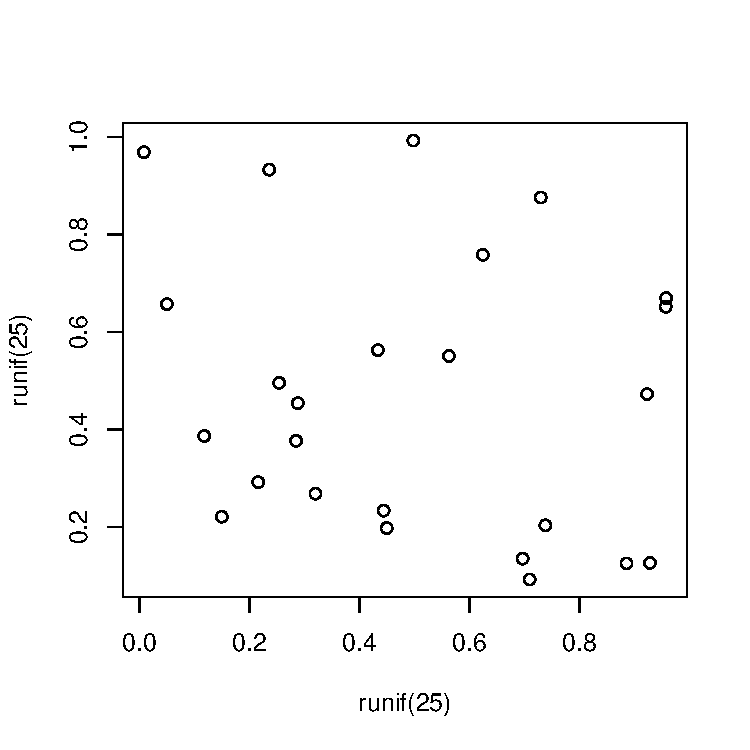
\includegraphics[width=0.5\linewidth]{BLS_EP_files/figure-latex/fig2-1} 

}

\caption{\label{fig2}A meaningless scatterplot.}\label{fig:fig2}
\end{figure}

\hypertarget{tables-coming-from-r}{%
\section{Tables coming from R}\label{tables-coming-from-r}}

Tables can also be generated using R chunks, as shown in Table
\ref{tab1} for example.

\begin{Shaded}
\begin{Highlighting}[]
\NormalTok{knitr}\SpecialCharTok{::}\FunctionTok{kable}\NormalTok{(}\FunctionTok{head}\NormalTok{(mtcars)[,}\DecValTok{1}\SpecialCharTok{:}\DecValTok{4}\NormalTok{], }
    \AttributeTok{caption =} \StringTok{"}\SpecialCharTok{\textbackslash{}\textbackslash{}}\StringTok{label\{tab1\}Caption centered above table"}
\NormalTok{)}
\end{Highlighting}
\end{Shaded}

\begin{longtable}[]{@{}lrrrr@{}}
\caption{\label{tab1}Caption centered above table}\tabularnewline
\toprule
& mpg & cyl & disp & hp \\
\midrule
\endfirsthead
\toprule
& mpg & cyl & disp & hp \\
\midrule
\endhead
Mazda RX4 & 21.0 & 6 & 160 & 110 \\
Mazda RX4 Wag & 21.0 & 6 & 160 & 110 \\
Datsun 710 & 22.8 & 4 & 108 & 93 \\
Hornet 4 Drive & 21.4 & 6 & 258 & 110 \\
Hornet Sportabout & 18.7 & 8 & 360 & 175 \\
Valiant & 18.1 & 6 & 225 & 105 \\
\bottomrule
\end{longtable}

\renewcommand\refname{References}
\bibliography{mybibfile.bib}


\end{document}
